\documentclass[conference, onecolumn]{IEEEtran}
\IEEEoverridecommandlockouts

% Packages
\usepackage{cite}
\usepackage{amsmath,amssymb,amsfonts}
\usepackage{algorithmic}
\usepackage{graphicx}
\usepackage{textcomp}
\usepackage{xcolor}
\usepackage{flushend}
\usepackage{titlesec}
\usepackage{float} % <-- To use [H] for figures

% Font size adjustment
\usepackage{anyfontsize}
\usepackage{lmodern}
\renewcommand{\normalsize}{\fontsize{13}{15}\selectfont}
\renewcommand{\small}{\fontsize{12}{14}\selectfont}
\renewcommand{\footnotesize}{\fontsize{11}{13}\selectfont}

\def\BibTeX{{\rm B\kern-.05em{\sc i\kern-.025em b}\kern-.08em
    T\kern-.1667em\lower.7ex\hbox{E}\kern-.125emX}}

\begin{document}

\title{Development of a Bluetooth-Controlled IoT-Based Smart Home System for Energy Efficiency and Security}

\author{
Tran Dinh Thien, Nguyen Phu Cuong, Nguyen Huynh Nhat Thinh, Truong Doan Anh Khoa\\
FPT University, Ho Chi Minh Campus, Vietnam\\
 ducdnm2@fe.edu.vn
}

\maketitle

\begin{abstract}
This paper introduces the design and development of a smart home system powered by Internet of Things (IoT) technologies. The system leverages Bluetooth and Wi-Fi connectivity to enhance automation, energy efficiency, and home security. Through a combination of microcontrollers (Arduino Uno and ESP32), various environmental sensors, and a web-based interface, the proposed system enables real-time monitoring and control of home appliances and conditions. Experimental validation demonstrates the system's ability to automate responses to environmental inputs, authorize user access through RFID, and allow remote control through a web platform. The paper concludes with discussions on results, limitations, and future improvement directions.
\end{abstract}

\section{Introduction}
The modern home increasingly integrates intelligent technologies to enhance user convenience, improve safety, and optimize energy consumption. Internet of Things (IoT) solutions offer homeowners the capability to monitor and control home functions from remote locations using smart devices. However, many existing systems are limited by high implementation costs or lack of customization.

This project aims to build a cost-effective, modular smart home system using open-source microcontrollers and standard communication protocols. The system architecture includes Bluetooth-enabled Arduino and Wi-Fi-enabled ESP32 to manage home access, monitor environmental parameters, and communicate with a cloud-based or local web application.

Our design objectives include:
\begin{itemize}
    \item Enable secure access using RFID verification.
    \item Monitor environmental conditions (e.g., motion, gas, obstacles).
    \item Provide automation through sensor-triggered events.
    \item Facilitate manual overrides via a responsive web interface.
\end{itemize}

\begin{figure}[H]
\centering
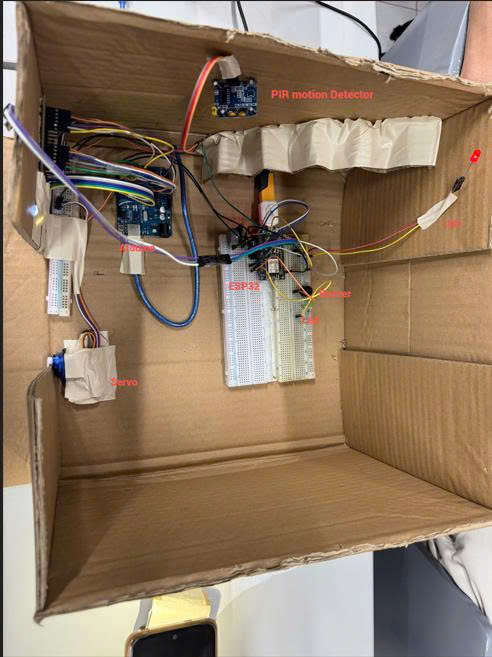
\includegraphics[width=0.8\linewidth]{IntroImg.png}
\caption{First part: Smart home concept illustration.}
\label{fig:intro_image1}
\end{figure}

\begin{figure}[H]
\centering
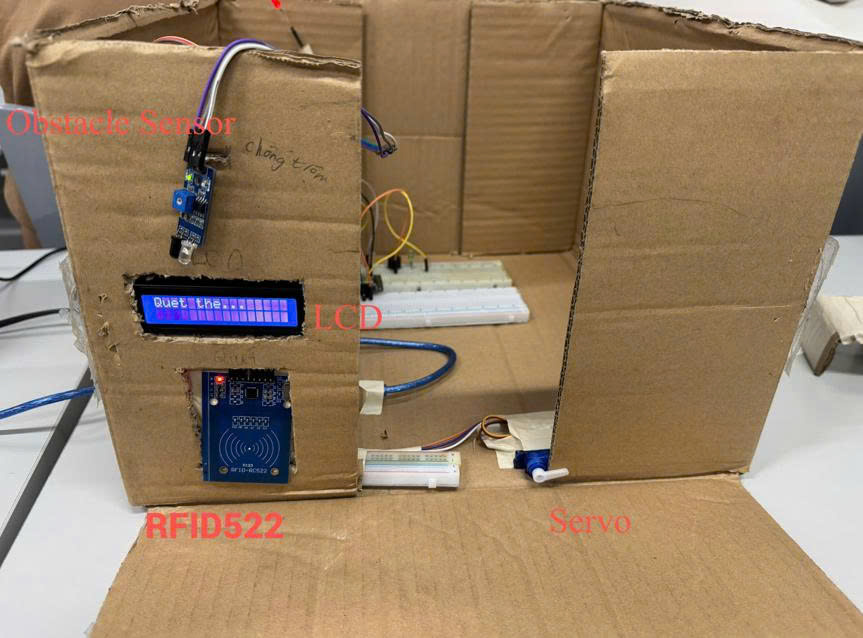
\includegraphics[width=0.8\linewidth]{IntroImg2-fotor-20250724142914.png}
\caption{Second part}
\label{fig:intro_image2}
\end{figure}


\section{Background and Literature Review}
Smart home systems have evolved significantly with the rise of IoT. Systems like Nest and SmartThings have introduced remote control and automation for lights, thermostats, and locks. However, these solutions often require proprietary hardware or cloud subscriptions.

Open-source platforms such as Arduino and ESP32 allow for more affordable and customizable alternatives. Prior research has demonstrated the feasibility of using Arduino in access control systems with RFID, while ESP32’s wireless capabilities make it ideal for networked applications. This project builds upon such literature by integrating both technologies into a cohesive home automation prototype.

\section{System Design Overview}

\begin{figure}[H]
    \centering
    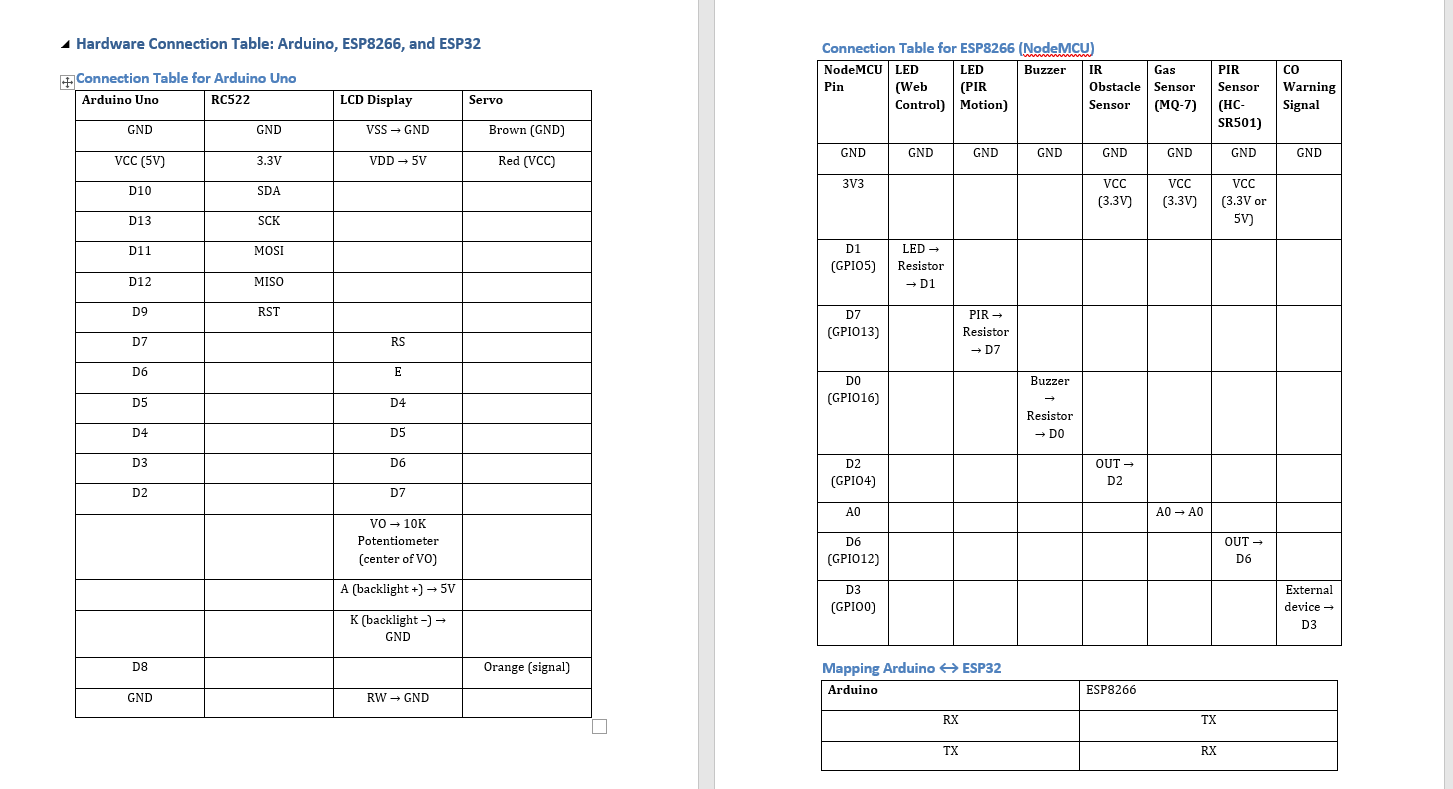
\includegraphics[width=0.8\linewidth]{Table.png} 
    \caption{System design showing communication between Arduino Uno and ESP32, and connected components.}
    \label{fig:system_overview}
\end{figure}

The proposed system includes two main processing units:
\begin{itemize}
    \item \textbf{Arduino Uno}: Handles RFID-based access control, LCD notifications, and servo actuation.
    \item \textbf{ESP32}: Collects data from sensors and communicates with a mobile/web interface via Wi-Fi.
\end{itemize}

Interconnected sensors and actuators include:
\begin{itemize}
    \item PIR motion detector
    \item CO (carbon monoxide) sensor
    \item Obstacle detection sensor
    \item Buzzer and LEDs for alerts
\end{itemize}

Communication between Arduino and ESP32 is enabled via serial interface, ensuring modular control and data sharing.

\section{Block Diagram and Architecture}
Figure~\ref{fig:block} shows the overall interaction between hardware components in the system.

\begin{figure}[H]
\centering
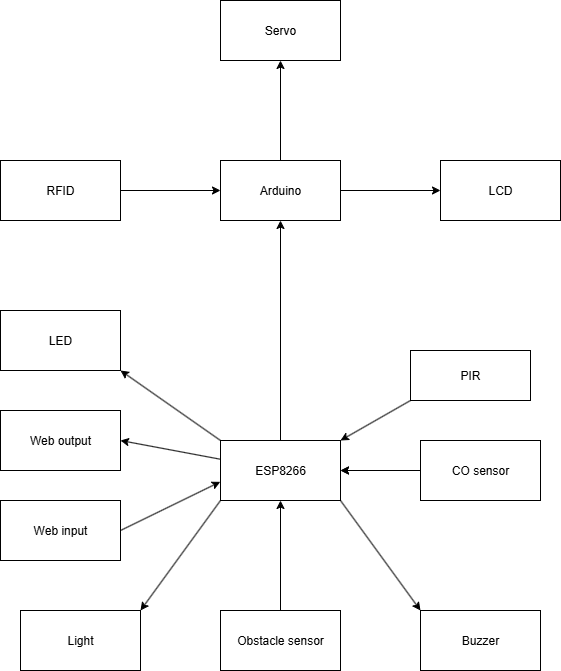
\includegraphics[width=0.95\linewidth]{Block_diagram.png}
\caption{System block diagram.}
\label{fig:block}
\end{figure}

The RFID reader communicates with Arduino to verify access. If verified, it triggers the servo motor to unlock the door. Sensor data from the environment is processed by ESP32, which acts accordingly and updates the status via web interface.

\section{Hardware Description}
\subsection{Component List}
\begin{itemize}
    \item \textbf{Arduino Uno } — Main microcontroller for RFID and servo control.
    \item \textbf{ESP32 Dev Kit} — Handles sensing and wireless communication.
    \item \textbf{RFID Reader (MFRC522)} — For access control.
    \item \textbf{Servo Motor} — To control locking mechanism.
    \item \textbf{LCD 16x2 Display} — Displays status of access attempts.
    \item \textbf{PIR Sensor} — Detects motion within range.
    \item \textbf{CO Sensor} — Monitors indoor gas levels.
    \item \textbf{Obstacle Sensor} — Detects physical barriers or movement.
    \item \textbf{Buzzer and LEDs} — Alerts users of unsafe conditions.
\end{itemize}

\subsection{Circuit Schematic}
Figure~\ref{fig:circuit} demonstrates the connection layout between modules.

\begin{figure}[H]
\centering
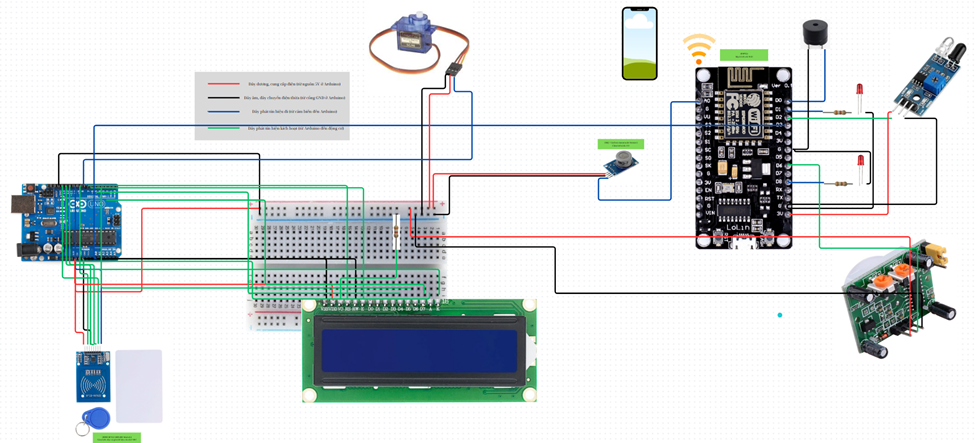
\includegraphics[width=0.95\linewidth]{circuit.jpg}
\caption{Hardware wiring diagram.}
\label{fig:circuit}
\end{figure}

\section{Software Development}
The Arduino code was written in the Arduino IDE using standard libraries for RFID, servo, and LCD communication. The firmware listens for RFID inputs, compares tags with authorized UIDs, and then sends success/failure messages to the LCD and ESP32.

ESP32 firmware, programmed via the Arduino framework, handles:
\begin{itemize}
    \item Reading values from sensors
    \item Making decisions based on thresholds
    \item Hosting a web interface on local Wi-Fi network
    \item Activating buzzer/LEDs on abnormal events
\end{itemize}

\subsection{Flowchart}
Figure~\ref{fig:flowchart} illustrates the software's logic.

\begin{figure}[H]
\centering
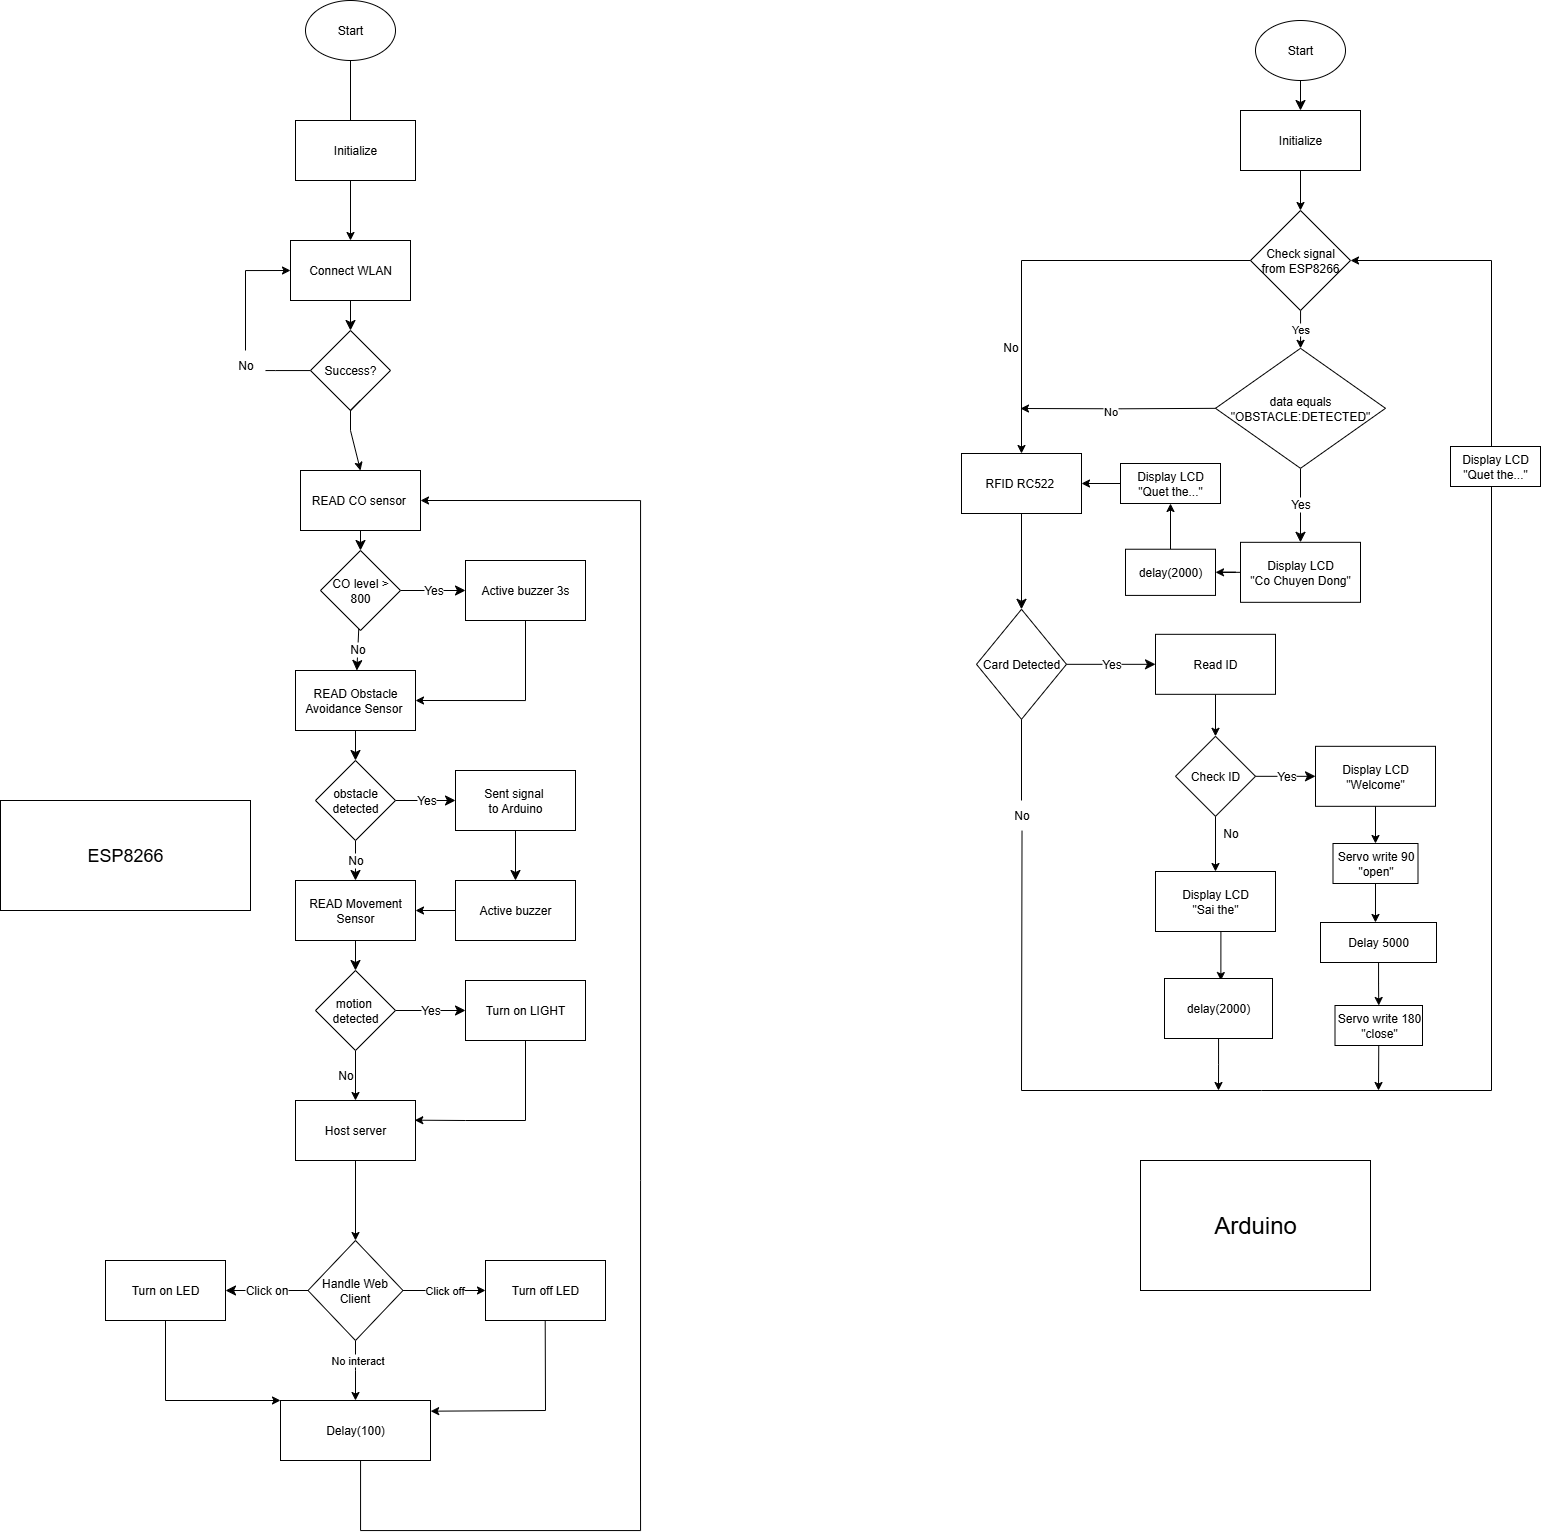
\includegraphics[width=0.95\linewidth]{Flowchart.drawio.png}
\caption{Software operation flowchart.}
\label{fig:flowchart}
\end{figure}

\section{Prototype Assembly and Testing}
\subsection{Assembly Process}
The prototype was constructed on a breadboard. Components were wired according to the schematic. The RFID reader and servo were placed to simulate a door lock, while sensors were fixed at representative positions (e.g., door, hallway).

\subsection{Functional Testing}
Multiple tests were performed:
\begin{itemize}
    \item RFID authentication: Valid tags granted access; invalid tags were denied.
    \item Motion detection: Triggered ESP32 to start web server.
    \item CO sensor: Buzzer activated when levels exceeded threshold.
    \item Obstacle sensor: Alerts user when objects approach critical zones.
    \item Remote toggling: From web interface, users could activate LEDs.
\end{itemize}

\section{Results and Observations}
The system successfully performed real-time access control, environmental sensing, and user interface interaction. The response times were within 1–2 seconds, and sensor triggers were consistent.

Issues observed:
\begin{itemize}
    \item Wi-Fi instability occasionally delayed interface loading.
    \item RFID reader sensitivity varied with distance and tag orientation.
\end{itemize}

\section{Discussion}
Our smart home prototype demonstrates a practical use of open-source platforms for real-world applications. Its modular nature allows for easy integration of new sensors or features. However, further refinements are needed:
\begin{itemize}
    \item \textbf{Security}: Current system lacks encryption; future versions should use HTTPS or VPN tunneling.
    \item \textbf{Scalability}: For multi-room homes, additional ESP32s or mesh networking should be used.
    \item \textbf{Cloud Storage}: Logging sensor data would help in analytics and long-term monitoring.
\end{itemize}

\section{Reference Document}
\begin{itemize}
    \item \textbf{Chat GPT}
    \item \textbf{Youtube}: https://www.youtube.com/watch?v=qyl4SEGSqKM
    \item \textbf{Youtube}: https://www.youtube.com/watch?v=gZ4hLL-SfdA
    
\end{itemize}

\section{Conclusion}
This project achieved its goal of creating a functional, affordable smart home system using ESP32 and Arduino. The dual-controller architecture enabled real-time automation and responsive remote control. Results validate its use in basic home automation and pave the way for expanded implementations.

\section{Future Work}
To enhance system functionality and reliability, we recommend the following future developments:
\begin{itemize}
    \item Implement two-factor authentication for secure access.
    \item Add camera modules for video monitoring.
    \item Transition to cloud-based dashboard with user login.

\end{itemize}

\section{Author Contributions}
\begin{table}[H]
\centering
\caption{Team member contributions}
\begin{tabular}{|c|c|c|c|}
\hline
\# & Name & Task & Contribution \\
\hline
1 & Tran Dinh Thien & Flowchart, diagrams & 25\% \\
2 & Nguyen Phu Cuong & System architecture & 25\% \\
3 & Nguyen Huynh Nhat Thinh & Programming, testing & 25\% \\
4 & Truong Doan Anh Khoa & Documentation, editing & 25\% \\
\hline
\multicolumn{3}{|c|}{\textbf{Total}} & 100\% \\
\hline
\end{tabular}
\end{table}

\end{document}